\documentclass[uplatex, dvipdfmx, 12pt]{beamer}
\usepackage[12pt]{moresize}
\usepackage{xcolor}
\usepackage{tcolorbox}
\usepackage{bxdpx-beamer}
\usepackage{pxjahyper}
\usepackage{listings,jlisting}
\usepackage{amsmath, newtxmath}
\usepackage{underscore}
\usepackage{setspace}
\usepackage{float} \renewcommand{\kanjifamilydefault}{\gtdefault}
\usetheme{Rochester}
\usecolortheme{seahorse}
%\usetheme{metropolis}
\usefonttheme{professionalfonts} 
\usefonttheme[onlymath]{serif}
\setbeamertemplate{navigation symbols}{}
%\setbeamerfont{page number in head/foot}{size=\small}
\setbeamertemplate{footline}[frame number]
\newcommand{\source}[1]{{\vskip0pt plus 1filll \scriptsize #1}}
\usepackage{import}
\usepackage{xifthen}
\usepackage{pdfpages}
\usepackage{transparent}
\newcommand{\incfig}[1]{
  \def\svgwidth{\columnwidth}
  \import{./figures/}{#1.pdf_tex}
}
\newcommand{\incsmfig}[1]{
  \def\svgwidth{\columnwidth/2}
  \import{./figures/}{#1.pdf_tex}
}
\usepackage[absolute,overlay]{textpos}
\title{\bfseries Linux講習会}
\author{長谷川央}
\institute{三重大学 工学部\\情報工学科}
\date{2019-05-30}
\keywords{Linux}
\begin{document}
{
  \setbeamertemplate{footline}{}
  \maketitle
}
\begin{frame}{目次}
  % 本題は軽く,ここでコラムの存在を伝える
  \setbeamertemplate{section in toc}[sections numbered]
  \tableofcontents
\end{frame}

\section{講習会の目標}
\begin{frame}{講習会の目標}
  % この時点ではパイプが何か分からなくても大丈夫です.
  % パイプはLinuxの特徴を色濃く反映していてとても重要で有用なものです.
  % この講習会が終わった後には,パイプを扱えるようになってもらいたいと考えています.
  \begin{LARGE}パイプをマスターする!\end{LARGE}
\end{frame}

\section{Linuxについて}
\begin{frame}{Linux}
  \begin{block}{Linuxとは}
  \begin{itemize}
    \setlength\itemsep{1em}
    \item Unix系OSの1つ
    \item 一部企業用を除き無料
    \item 動作が軽いことで有名
    \item カスタマイズ性が非常に高い
    \item Wi-Fiルータ,プリンタ,ロケット制御用のシステム,スーパーコンピュータなど様々な用途で使われている
  \end{itemize}
\end{block}
\end{frame}
\begin{frame}{OS (オペレーティング・システム) }
  OS (オペレーティング・システム) : \\コンピュータの一番の基礎となるソフトウェアのこと. 
  
  \vspace{1em} 
  \begin{block}{OSの例}
  \begin{itemize}
    \setlength\itemsep{1em}
    \item Windows
    \item macOS
    \item Linux
  \end{itemize}
  \end{block}

  \pause
  \vspace{1em}
  \begin{Large}→\textcolor{red}{OSが変わると見た目や使い方が\\\hspace{1em}変わる!}\end{Large}
\end{frame}

\begin{frame}{Windowsの見た目}
  \begin{center}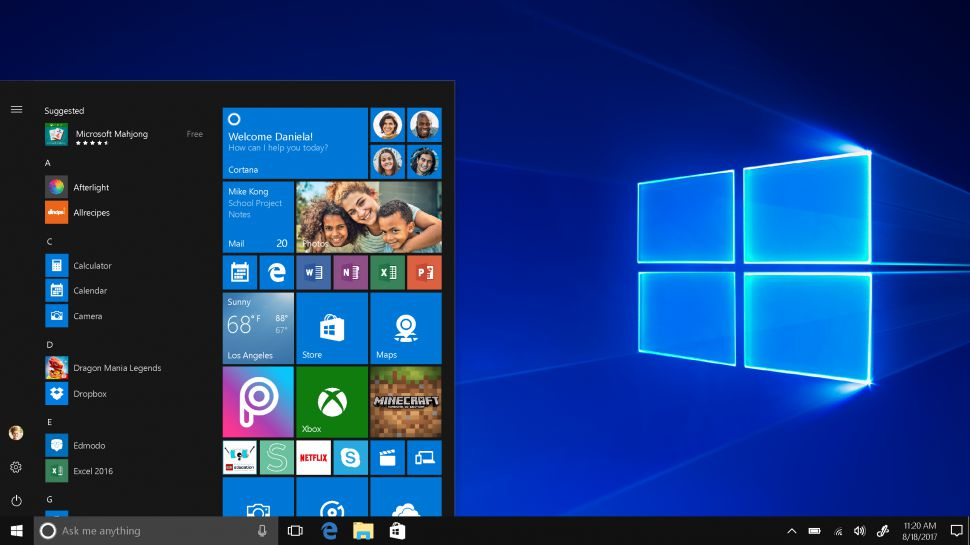
\includegraphics[width=\textwidth]{./figures/Windows.jpg}\end{center}
  \source{https://www.techradar.com/news/windows-10-cloud-release-date-news-and-rumors}
\end{frame}
\begin{frame}{Linuxの見た目 (1/4)}
  % KDE
  \begin{center}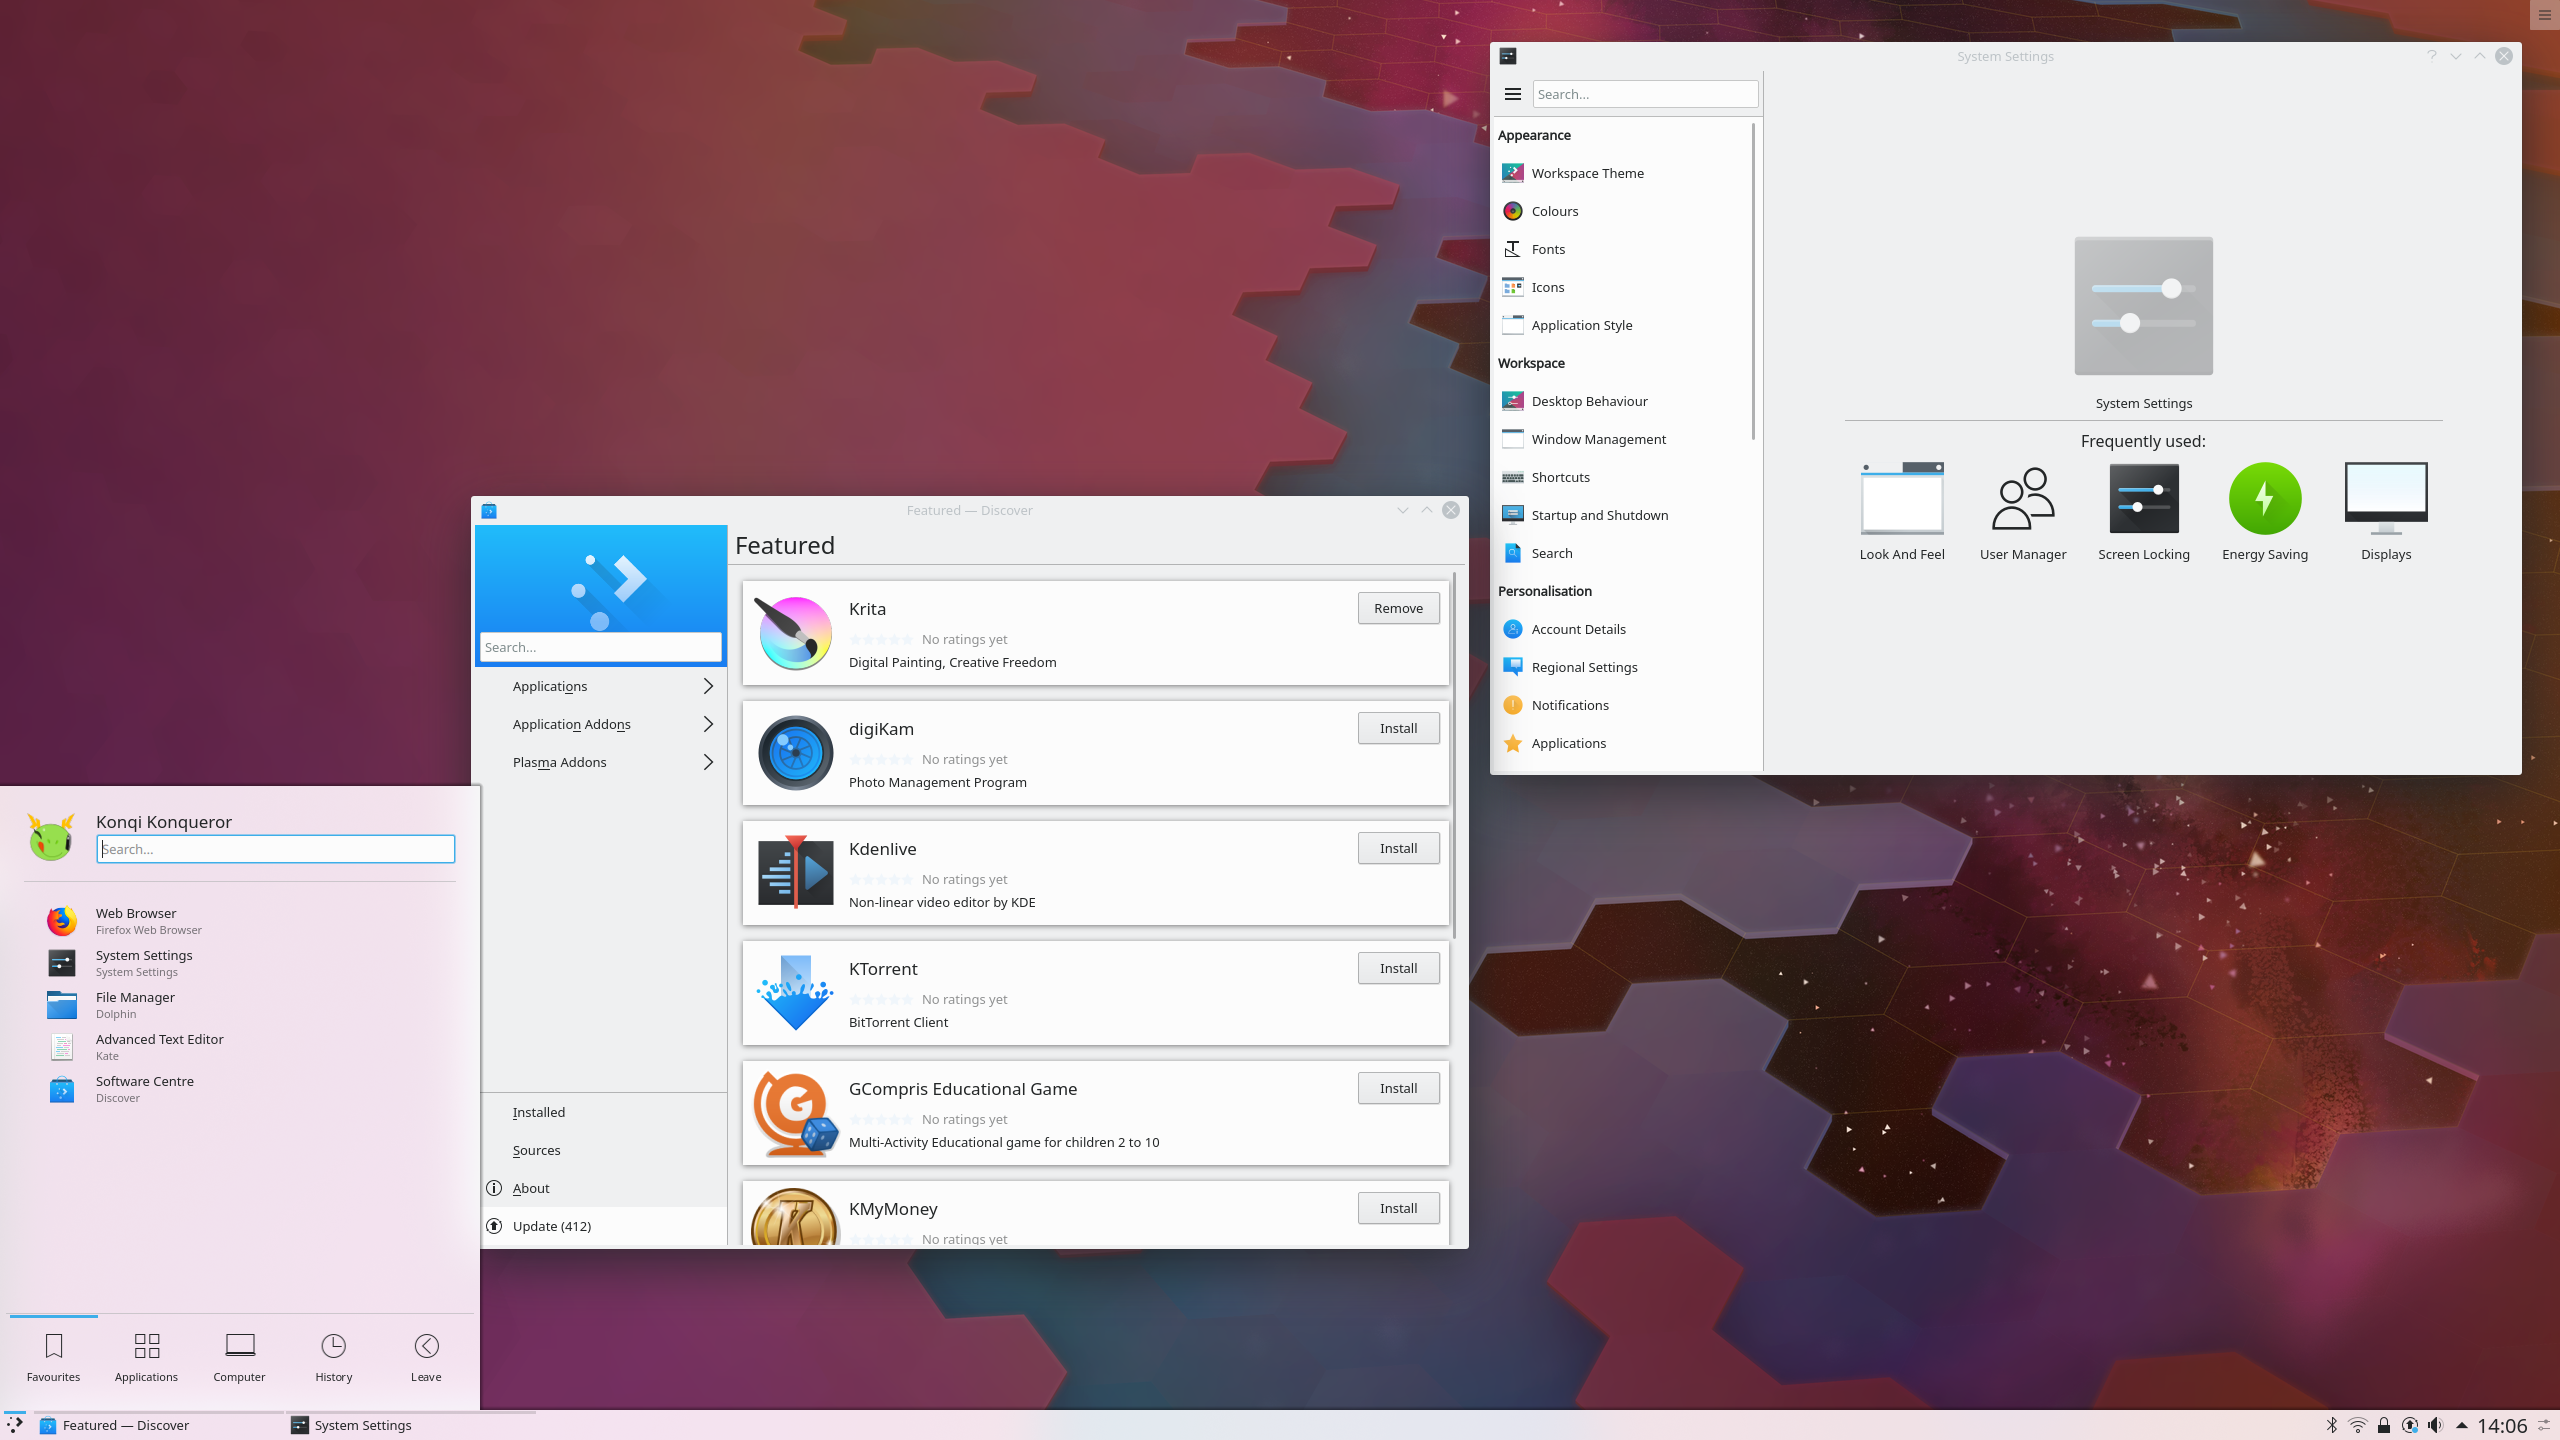
\includegraphics[width=\textwidth]{./figures/Plasma.png}\end{center}
  \source{https://kde.org/announcements/plasma-5.15.0.php}
\end{frame}
\begin{frame}{Linuxの見た目 (2/4)}
  \begin{center}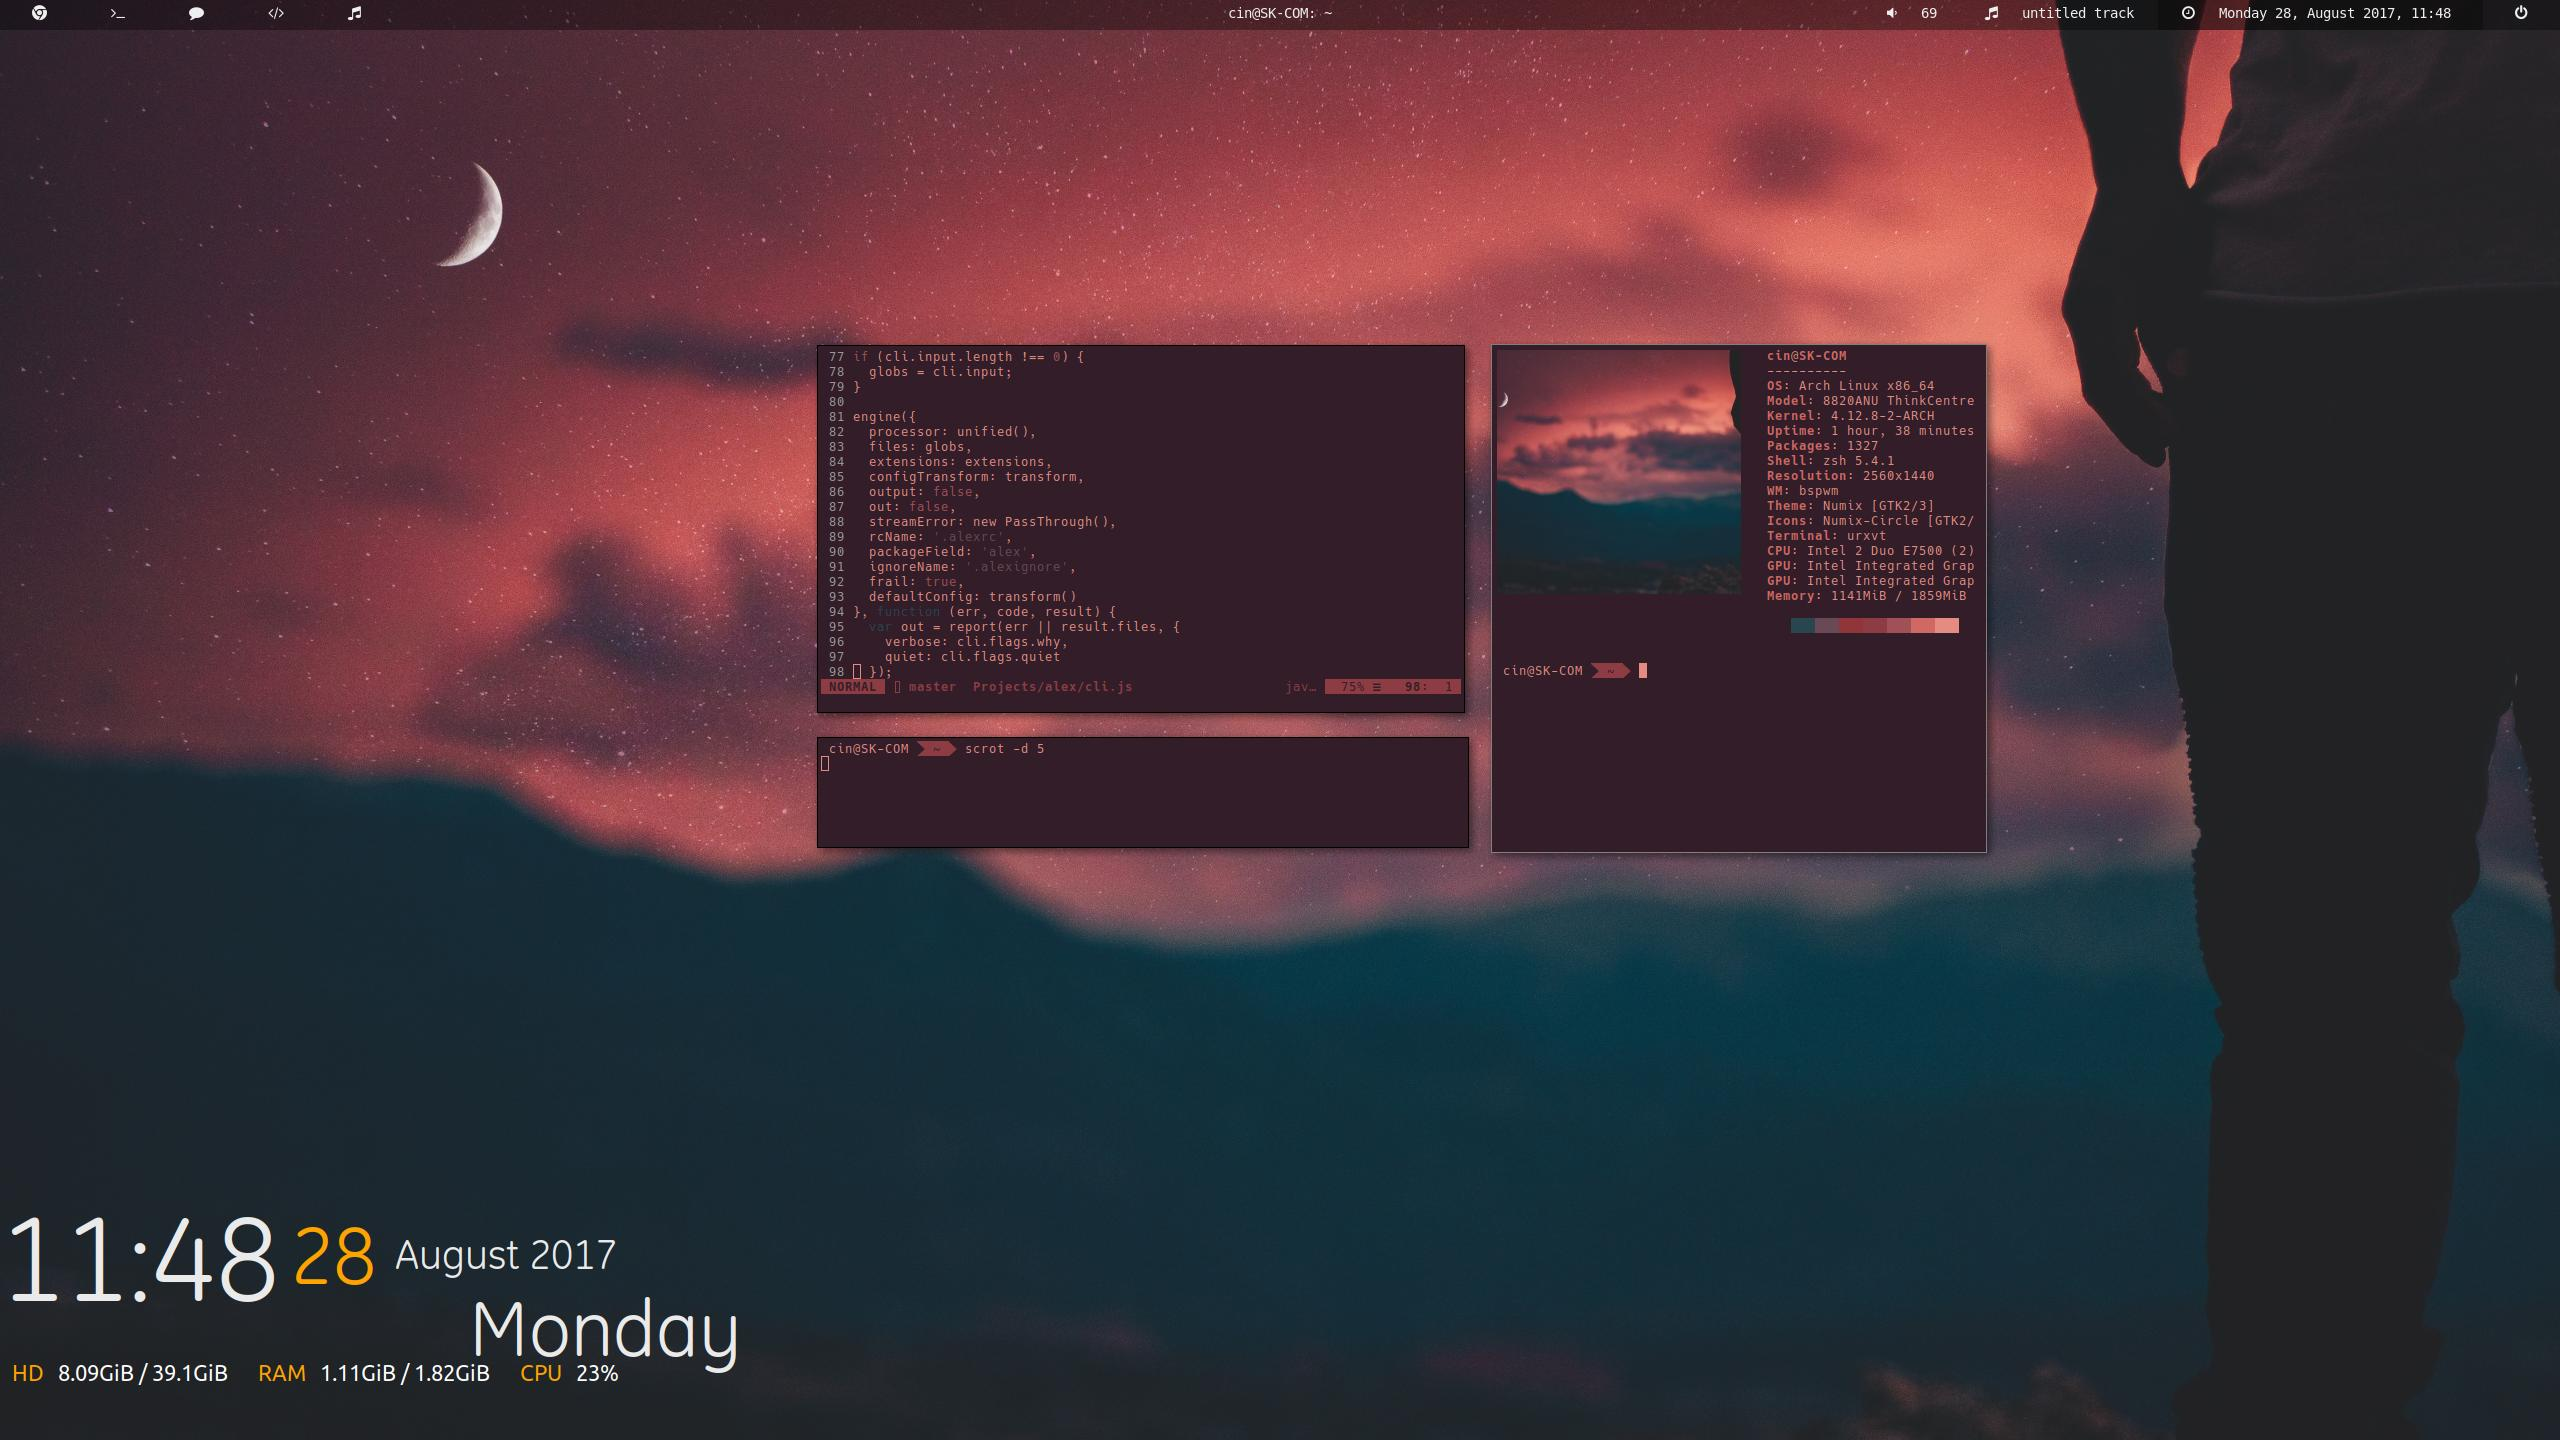
\includegraphics[width=\textwidth]{./figures/bspwm.jpg}\end{center}
  \source{https://imgur.com/r/unixporn/OF3ZI}
\end{frame}
\begin{frame}{Linuxの見た目 (3/4)}
  \begin{center}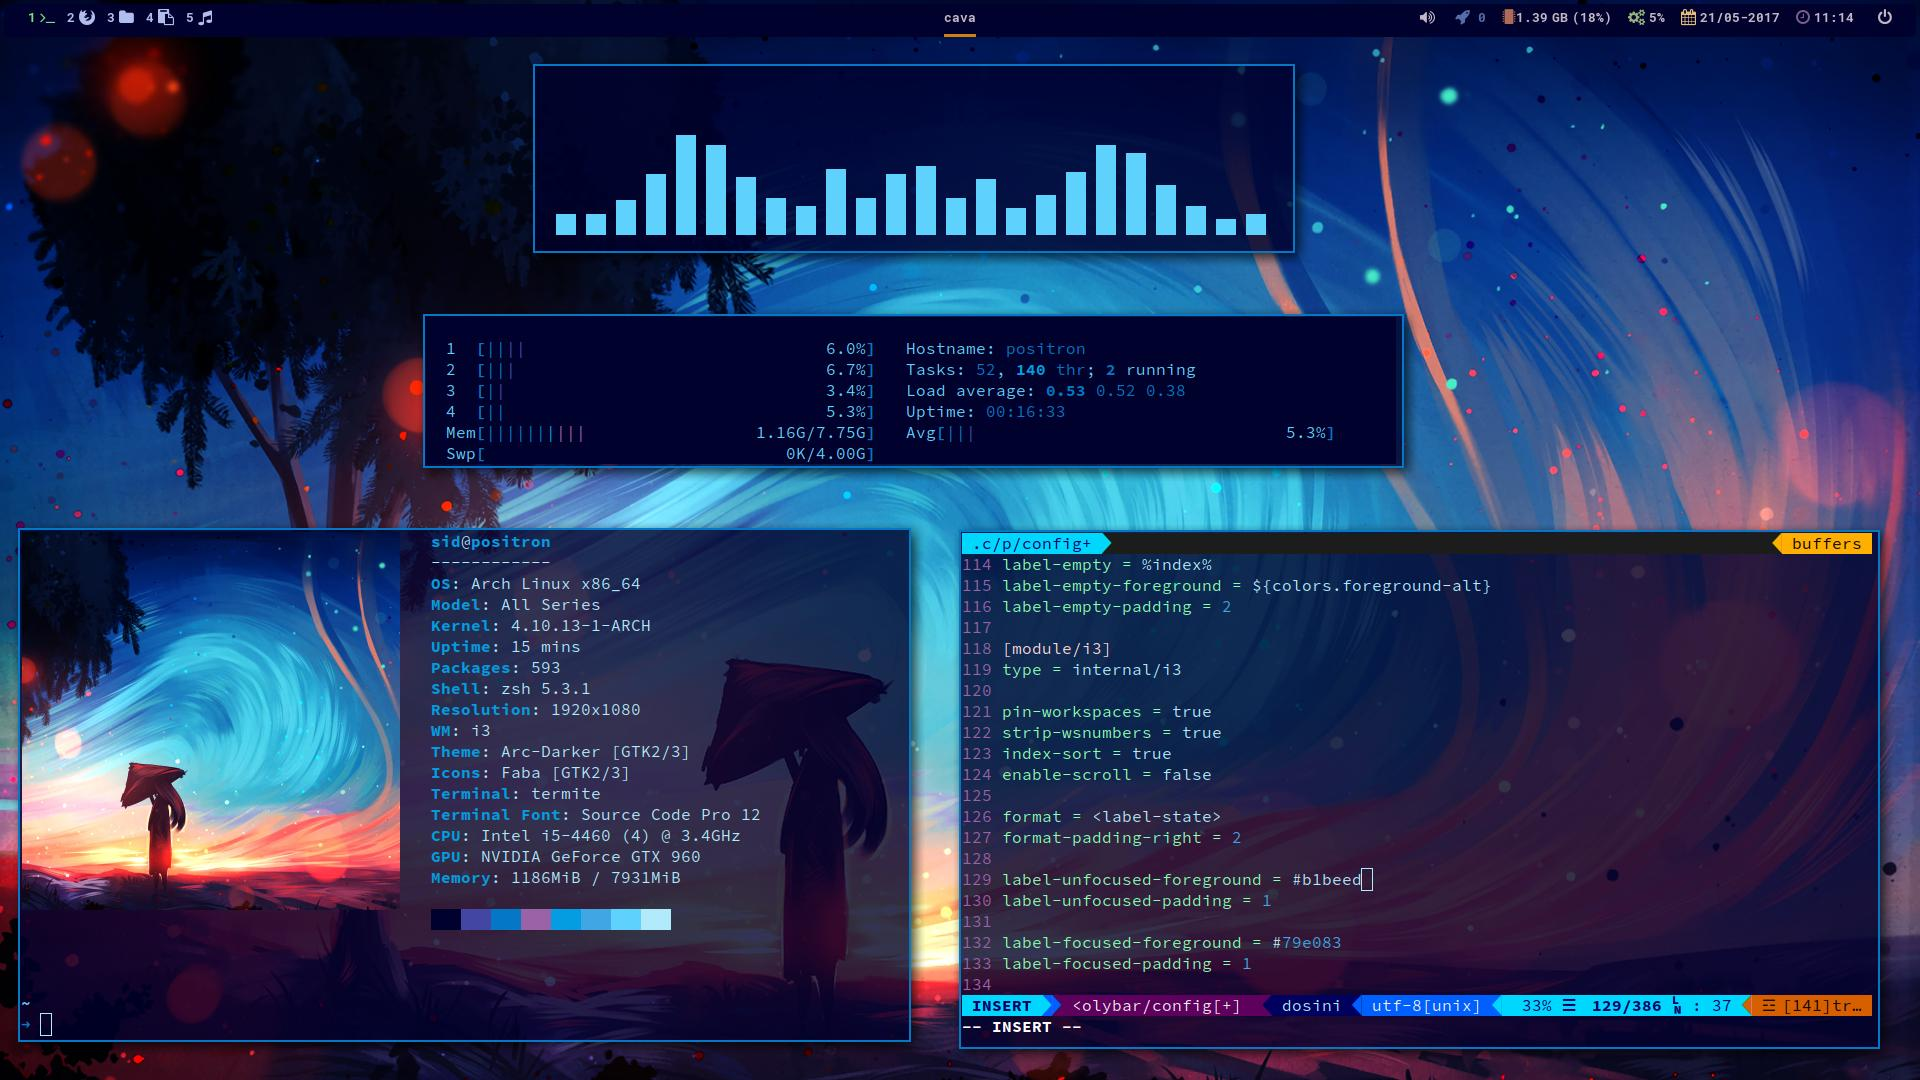
\includegraphics[width=\textwidth]{./figures/LinuxRice.jpg}\end{center}
\source{https://imgur.com/TNIcUw2}
\end{frame}
\begin{frame}{Linuxの見た目 (4/4)}
  % android
  \begin{center}
\includegraphics[height=0.9\textheight]{./figures/Android.png}\end{center}
    \source{https://en.wikipedia.org/wiki/File:Android_5.0-en.png}
\end{frame}
\begin{frame}{Linuxの特徴}
  Linuxは見た目を自由に変えられる
  
  \textcolor{red}{しかし,中身は同じ!}\\

  \vspace{1em}
  どのLinuxも『シェル』というプログラムを中心に\\動いている

  \pause
  \vspace{1em}
  \begin{Large}つまり...\\ \hspace{5em}シェルを極めれば\\\hspace{5em}どんなLinuxも\textcolor{red}{自由自在に}\\\vspace{0.4em}\hspace{5em}扱えるようになる!\end{Large}
\end{frame}

\section{シェルについて}
\begin{frame}{シェル (1/3)}
  \begin{Large}
  シェル :\\
    \vspace{1em}
  ユーザとOSを結びつけるための\\プログラム\end{Large}
\end{frame}
\begin{frame}{シェル (2/3)}
  % 端末の開き方
  % 「コマンドを入力する」という基本的な使い方の説明
  シェルを直接扱いたいときには 端末 (Terminal) を開く.
  \begin{center}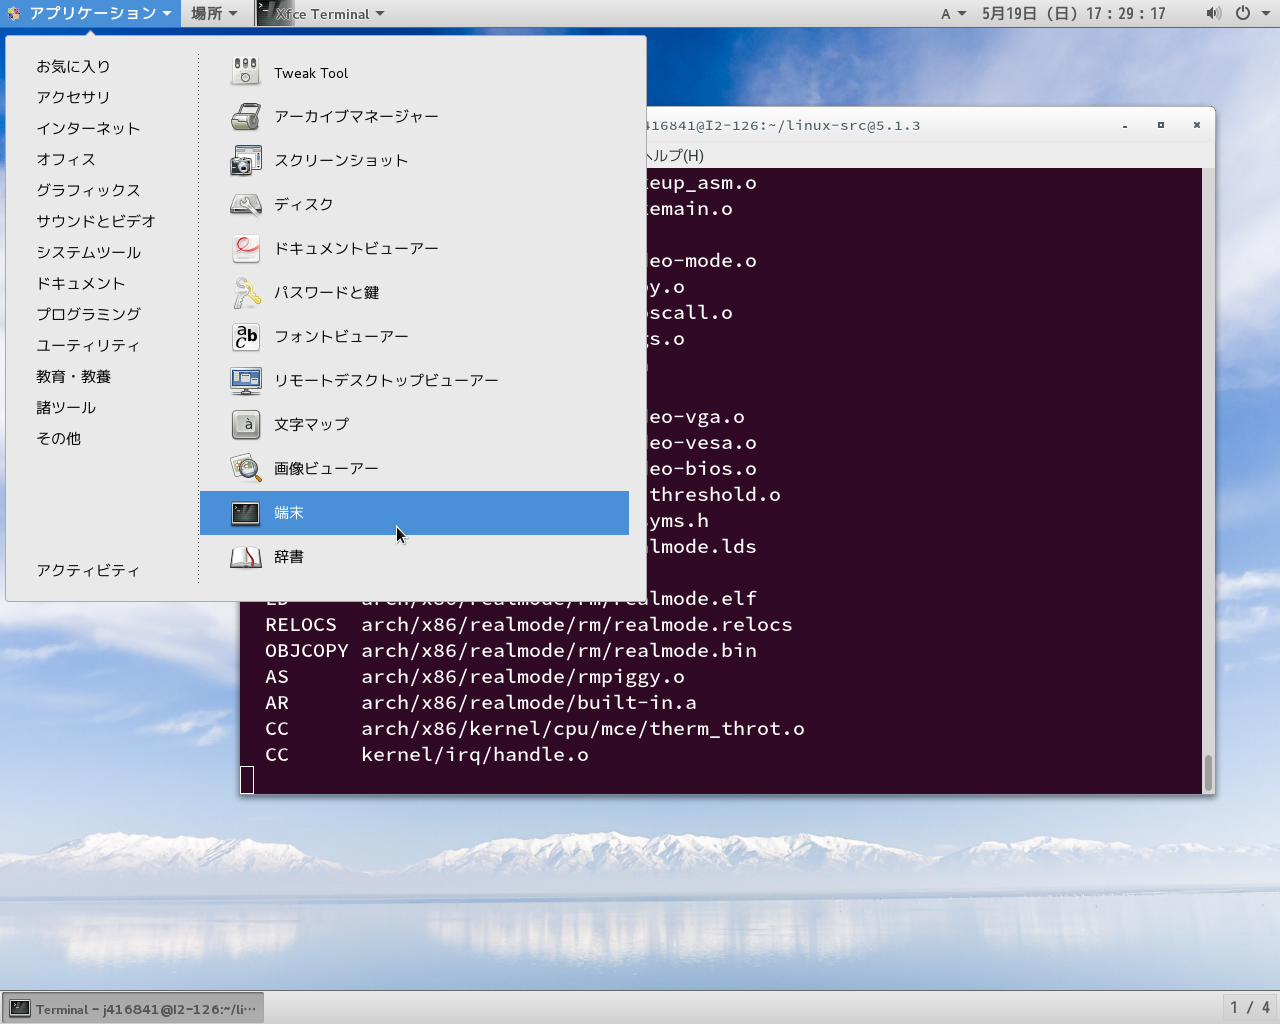
\includegraphics[height=0.9\textheight]{./figures/Terminal.png}\end{center}
\end{frame}

\defverbatim[colored]\lstShell{
  \begin{lstlisting}[language=bash,basicstyle=\small\ttfamily,xleftmargin=0zw]
  $ echo "Hello,World!"
\end{lstlisting}
}
\begin{frame}{シェル (3/3)}
  端末 (Terminal) にコマンドを打つことで\\
  シェルを使うことができる.

  \vspace{1em}
  例
  \begin{tcolorbox}
  \lstShell
  \end{tcolorbox}
  注意:先頭の\$は入力しない.
\end{frame}

\begin{frame}{シェルを極めるために}
  %では,何をすればシェルを極められるのか
  %パイプを極める=シェルを極める 
  \begin{large}
  Q. シェルを極めるにはどうすればよいか?
  
  \pause
    \vspace{2em}
  A. まずは\textcolor{red}{パイプをマスターする}こと!
  \end{large}
\end{frame}
\defverbatim[colored]\lstpipe{
  \begin{lstlisting}[language=bash,basicstyle=\ssmall\ttfamily,xleftmargin=-1.8zw]
$ command1 | command2 | command3 | ...
\end{lstlisting}
}

\begin{frame}{パイプ}
  % パイプとは何か
  パイプ :  \\
  $|$ の前のコマンドの出力を次のコマンドの入力とする仕組み 


  \vspace{1em}
  \begin{tcolorbox}
  \lstpipe
  \end{tcolorbox}

  \begin{block}{意味}
    command1の出力をcommand2へ入力として受け渡す.\\
    command2の出力をcommand3へ入力として受け渡す.\\
    command3の出力を...
  \end{block}
\end{frame}

\defverbatim[colored]\lstzip{
  \begin{lstlisting}[language=bash,basicstyle=\ssmall\ttfamily,xleftmargin=-1.8zw]
$ ls
$ ls | xargs -n1 -t -I{} zip -r {}.zip {}
\end{lstlisting}
}

\begin{frame}{パイプの使用例 zipファイル一括圧縮}
  複数のディレクトリを一括zip圧縮.\\
  次のコマンドを実行すると,ディレクトリ内のディレクトリが全てzip圧縮される.

  \vspace{1em}
  \begin{tcolorbox}
    \lstzip
  \end{tcolorbox}

\end{frame}

\defverbatim[colored]\lstpass{
  \begin{lstlisting}[language=bash,basicstyle=\ssmall\ttfamily,xleftmargin=-1.8zw]
$ tr -dc 'a-zA-Z0-9&%$#' < /dev/urandom
$ tr -dc 'a-zA-Z0-9&%$#' < /dev/urandom | fold -w 32
$ tr -dc 'a-zA-Z0-9&%$#' < /dev/urandom | fold -w 32 | head -n 1
\end{lstlisting}
}
\begin{frame}{パイプの使用例 パスワード自動生成}
  次のコマンドを実行すると,32文字のパスワードが自動生成される.
  
  \vspace{1em}
  \begin{tcolorbox}
    \lstpass
  \end{tcolorbox}
  ※ コマンドを途中で終了したい場合はCtrlとCを同時押し.
\end{frame}


\begin{frame}{なぜパイプ?}
  % 一度振り返ってシェルを極めるとはパイプを極めることというのを言う (再掲してもよいかも)
  % パイプにはUnix系OSの思想が色濃く反映されている.
  なぜパイプを極めることがシェルやLinuxをマスターする\\ことにつながるのか.

  \vspace{1em}
  \pause
  \begin{large}→ 
    \hspace{1em}\textcolor{red}{パイプにはUnix系OSの思想が\\\hspace{2em}色濃く反映されている!}
  \end{large}
\end{frame}

\section{UNIX哲学}
\begin{frame}{UNIX哲学 (1/2)}
  \begin{textblock*}{0.4\linewidth}(40pt,70pt)
    \centering
    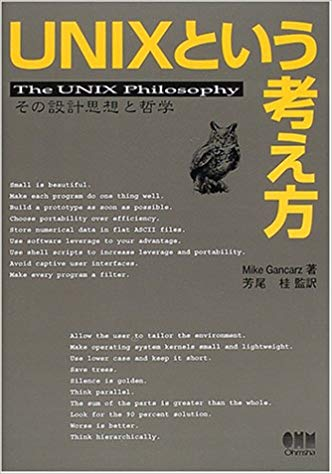
\includegraphics[width=\linewidth]{./figures/Unixph.jpg}
  \end{textblock*}
  \begin{textblock*}{0.6\linewidth}(160pt,70pt)
    \begin{itemize}
          \setlength\itemsep{2em}
      \item 2001年にオーム社から出版された
      \item 著者 Mike GancarzはX Window Systemの開発メンバー \\(グラフィックのソフトウェア)
      \item Unixの背後にある基本的な\\考え方について解説してある.
    \end{itemize}
  \end{textblock*}
\end{frame}
\begin{frame}{UNIX哲学 (2/2)}
  \begin{itemize}
    \setlength\itemsep{0.4em}
    \item \textcolor{red}{Small is beautiful. (小さいものは美しい)}
    \item \textcolor{red}{一つのプログラムには一つのことをうまくやらせる}
    \item できるだけ早く試作する
    \item 効率よりも移植性を優先する
    \item 数値データはASCIIフラットファイルに保存する
    \item \textcolor{red}{ソフトウェアを梃子 (てこ) として使う}
    \item シェルスクリプトによって梃子の効果と移植性を\\高める
    \item 過度の対話的インタフェースを避ける
    \item \textcolor{red}{すべてのプログラムをフィルタとして設計する}
  \end{itemize}
  %\source{Mike Gancarz (2001)『UNIXという考え方―その設計思想と哲学』(芳尾桂訳) オーム社.}
\end{frame}
\begin{frame}{Small is beautiful.}
  Unix系OSにおいて特に重視されている考え方.\\
  優れた機能を持つ大きなシステムやプログラムよりも,\\
  シンプルで分かりやすいプログラムを良い物だと評価する.

  \vspace{1em}
  \begin{block}{小さくすることの利点}
  \begin{itemize}
    \item シンプルなのでプログラムの使い方が分かりやすい.
    \item 保守・管理しやすい.
    \item 機能を増やしすぎて肥大化してしまうことを防げる.
    \item 他のプログラムと組み合わせやすくなる.
    \item 柔軟性が高くなる.
  \end{itemize}
  \end{block}
\end{frame}
\begin{frame}{一つのプログラムには一つのことを\\うまくやらせる}
  一つのプログラムだけで様々な処理を行えるようにしようとすると,機能が肥大化し,
  ユーザが把握できなくなってしまう.\\
  一つのプログラムに対して一つの役割を持たせることで次のような利点がある.

  \begin{block}{利点}
  \begin{itemize}
    \item 各プログラムを小さく保てる.
    \item 各プログラムの目的をユーザが把握しやすい.
    \item 他のプログラムと組み合わせやすくなる. 
  \end{itemize}
  \end{block}

\end{frame}
\begin{frame}{ソフトウェアを梃子 (てこ) として使う}
  自分でプログラミングをするよりも,洗練された既存の\\
  プログラムをツールとして (テコとして) 使うのが好ましい.

  \begin{block}{解釈}
  \begin{itemize}
    \item 自分でプログラミングをするよりもコマンドをうまく使うほうが効率のよい処理を行える.
    \item 自分でプログラミングをしなくても良いので時間を\\大幅に削減できる.
    \item コマンドをツールとして組み合わせることで簡単に\\自動化を実現できる.
  \end{itemize}
  \end{block}
\end{frame}
\begin{frame}{すべてのプログラムをフィルタとして設計する}
  フィルタというのはまさにパイプのことを指している.\\
  プログラムを入力に対して順に処理を行い,
  求めたい出力を得る仕組みだと考える.

  \begin{block}{利点}
    \begin{itemize}
      \item 小さなプログラムの組み合わせで大きな処理を行える.
      \item 処理内容を把握しやすくなる.
      \item フィルタを一部変えるだけで他の用途に転用できる.
    \end{itemize}
  \end{block}
\end{frame}

\begin{frame}{この講習会におけるUNIX哲学}
  \begin{itemize}
    \setlength\itemsep{2em}
    \item 原則,コマンドは1つのことをうまくやれるように\\設計されている.
    \item コマンドを梃子 (てこ) として自分の目的の達成に\\役立てると効率よく処理を行える.
    \item コマンドを組み合わせて,フィルタとして使うことで様々な処理を行える.
  \end{itemize}
\end{frame}

\section{演習の準備}

\defverbatim[colored]\lstInit{
  \begin{lstlisting}[language=bash,basicstyle=\ssmall\ttfamily,xleftmargin=-1.8zw]
$ git clone https://github.com/AkiraHasegawa1997/Linux_Workshop.git
$ cd Linux_Workshop
$ source init.sh
\end{lstlisting}
}

\begin{frame}{演習のための準備}
  初めに次の3行を実行してください.\\
  ※ 先頭の`\$'は入力しないでください.
  \vspace{1em}

  \begin{tcolorbox}
  \lstInit
  \end{tcolorbox}

  \vspace{1em}
  端末 (Terminal) を開き直したときは下2行を\\
  再実行してください.

  2つ目の端末を開くときも同様に下2行を\\実行してください.
\end{frame}

\defverbatim[colored]\lstTree{
  \begin{center}
\begin{lstlisting}[basicstyle=\small\ttfamily,xleftmargin=3zw]
Linux_Workshop
  ├── exercises
  │   ├── ex01
  │   │     └── ex01.txt
  │   ├── ex02
  │   │     ├── ex02.txt
  │   │     └── ex02.sh
  │   └── [...]
  ├── init.sh
  └── slides
      ├── figures
      └── slide.pdf
\end{lstlisting}
  \end{center}
}
\begin{frame}{演習の進め方}
  % パイプを使った演習がどこから始まるかを話す
  % パイプを意識してほしいことを強調
  \lstTree
\end{frame}
\begin{frame}{演習のための予備知識}
  % ディレクトリの説明をする?
  \begin{itemize}
    \setlength\itemsep{1em}
    \item pwd   : 現在いる場所を表示
    \item ls    : 現在いるディレクトリ (フォルダ) の中身の表示
    \item cd \textit{dir_name}  : ディレクトリ間の移動
    \item cd .. : 一つ上のディレクトリへ移動
    \item cat \textit{file_name}  : ファイルの内容の表示
    \item nano -w \textit{file_name} : ファイルを編集
  \end{itemize}
\end{frame}
\section{演習}
\end{document}
